\documentclass[10pt,a4paper]{article}
\usepackage{amsmath,amssymb,amsthm,graphicx}
\usepackage{amsmath,amssymb,amsthm,graphicx,xcolor,enumitem,ytableau}
\usepackage[a4paper,margin=24mm]{geometry}
\usepackage[colorlinks=true,linkcolor=blue,citecolor=blue,urlcolor=blue]{hyperref}
\newtheorem{theorem}{Theorem}[section]
\newtheorem{prop}[theorem]{Proposition}
\newtheorem{lemma}[theorem]{Lemma}
\newtheorem{coro}[theorem]{Corollary}
\theoremstyle{definition}
\newtheorem{defi}[theorem]{Definition}
\newtheorem{exam}[theorem]{Example}
\newtheorem{rema}[theorem]{Remark}
\numberwithin{equation}{section}
\emergencystretch=3em
\makeatletter
\newlabel{ex:shuffleDiagram}{{1.3}{1120}{}{}{}}
\newlabel{subsec:TL-imm}{{2.4}{1128}{}{}{}}
\makeatother
\title{Shape-content preserving bijection between D-compatible standard tableaux and Yamanouchi shuffle tableaux (Proposition 2.13)}
\author{Chau Nguyen, Son Nguyen, Dora Woodruff}
\date{doi:10.5802/alco.502; CC BY 4.0}
\begin{document}
\maketitle
\noindent\textit{Editorial note.} One standalone Proposition2.13 is counted; four supporting proofs are not split.\par\medskip
\noindent\textit{Editorial note.} Theorem1.2 is not collected as a complete target because its separate inverse-standardization lemma is left to readers. No proof has been supplied for that omission.\par\medskip
\noindent\textit{Editorial note.} Original mathematical text, notation and examples are unchanged. The initial proof roadmap is followed by all four full author lemma proofs.\par\medskip
\noindent\textit{Editorial note.} Author figures are vector crops of the exact licensed published PDF, with original form sizes restored.\par\medskip
\noindent\textit{Editorial note.} Before first compilation, the unselected contextual Section2.4 page locator was verified as printed1128 and corrected; mathematical text unchanged.\par\medskip
\noindent\textit{Editorial scope.} Author material collection only; no source mathematics repair or formal admission.\par\medskip
\noindent\textit{Allowed standard prerequisites (editorial).}\begin{itemize}
\item Partitions, skew shapes, standard and semistandard Young tableaux. Ordinary tableau conventions and retained original Definitions2.1 and2.10. Only basic combinatorial objects; every new D-compatibility and reading rule is retained.
\item Shuffle-tableau lowering operators and Yamanouchi terminology. Original definitions and Corollary 2.7, native lines 194–298, citing Nguyen–Pylyavskyy, Temperley-Lieb crystals (2025). The actual rules are reproduced rather than treated as an opaque current core. The contextual LR counting theorem is not a substitute for the four selected author proofs.
\end{itemize}\medskip
\section*{Selected author proposition and attribution}
Chau Nguyen, Son Nguyen and Dora Woodruff, \emph{Shuffle Tableaux, Littlewood--Richardson Coefficients, and Schur Log-Concavity}, Algebraic Combinatorics 9 (2026), no.~4, 1119--1137, doi:10.5802/alco.502. Published 2 September 2026, CC BY 4.0.

One count only: the standalone shape--content preserving bijection of original Proposition 2.13. The four complete author proofs in Lemmas 2.14--2.17 are retained together, not counted separately. The proposition's initial ``Proof sketch'' is a roadmap to those fully included proofs.

The separate main coefficient formula in Theorem 1.2 is not counted here: its inverse-standardization bridge in Lemma 2.19 is left to readers in the source. No missing argument has been supplied. The chosen bijection does not require that bridge.

The mathematical text below is selected unchanged from the exact official journal TeX. Original labels, wording and examples, including notation slips, are retained without mathematical correction. Figure assets are faithful vector crops of their original forms in the licensed published PDF, not redrawn images. Two pointers to unselected explanatory sections keep their original numbers; they do not replace any selected proof step.

The article's citation keys and original numeric reference labels were recovered from its PDF destinations; reference facts were rendered from its official article page. Journal template and metadata layout were replaced with a standard wrapper. No independent mathematical certification or generated proof is claimed.

\setcounter{section}{1}
\setcounter{figure}{4}

\section{Littlewood--Richardson coefficients}

\subsection{Shuffle tableaux and crystal operators}

    First, we review the relevant background on shuffle tableaux and their crystal operators, as introduced in \cite{nguyen2025temperley}.

    \begin{defi}\label{def:shuffle}
        Given two skew shapes $\lambda/\mu$ and $\nu/\rho$, the \textit{shuffle diagram} $D$ of shape $(\lambda/\mu)\circledast(\nu/\rho)$ is constructed as follows.

        \begin{itemize}
            \item If $\lambda/\mu$ has a square in position $(i,j)$, then add into $D$ a square in position $(2i-1,2j-1)$.
            \item If $\nu/\rho$ has a square in position $(i,j)$, then add into $D$ a square in position $(2i,2j)$.
        \end{itemize}
        
        A \textit{shuffle tableau} of shape $(\lambda/\mu)\circledast(\nu/\rho)$ is a filling of the shuffle diagram of shape $(\lambda/\mu)\circledast(\nu/\rho)$ such that the entries are weakly increasing along the rows and strictly increasing along the columns. The \textit{weight} of a shuffle tableau $T$, denoted $\omega(T)$, is $\prod_{i\geq 1} x_i^{c_i}$, where $c_i$ is the number of $i$-entries in $T$.

        In addition, we say square $(r_1,c_1)$ is \textit{right of} square $(r_2,c_2)$ if $r_2 > r_1$ or $r_2 = r_1$ and $c_2 < c_1$. In particular, this means that in the reading order from left to right, bottom to top, square $(r_1,c_1)$ is right of square $(r_2,c_2)$. Then, we also say $(r_2,c_2)$ is \textit{left of} $(r_1,c_1)$.
    \end{defi}

    Observe that the squares in the same row or column of $D$ are exactly those on the same row or column of the Young diagram of either $\lambda/\mu$ or $\nu/\rho$. Thus, one can think of a shuffle tableau of shape $(\lambda/\mu)\circledast(\nu/\rho)$ as interlacing two SSYTs or shape $\lambda/\mu$ and $\nu/\rho$ (see Figure \ref{fig:shuffleTableau}). In particular, we have
    \[ \sum_{\substack{\text{$T$ of shape} \\ (\lambda/\mu)\circledast(\nu/\rho)}} \omega(T) = s_{\lambda/\mu}s_{\nu/\rho}. \]
    \begin{figure}[h!]
        \centering
        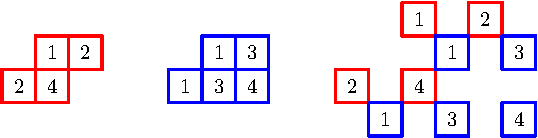
\includegraphics[scale = 0.8]{figures/shuffleTableau.pdf}
        \caption{SSYTs of shape $\lambda/\mu$ (left) and $\nu/\rho$ (center) and their corresponding shuffle tableau (right)}
        \label{fig:shuffleTableau}
    \end{figure}

    \begin{defi}
        Given a shuffle tableau $T$, an $(i,i+1)$-overlap is a pair of squares $(s,t)$ on the same column such that $s$ contains an $i$ and $t$ contains an $i+1$. We define the \textit{$i$-reading word} $w_i(T)$ as follows.
        
        \begin{enumerate}
            \item Consider only the squares containing $i$ and $i+1$.
            \item Remove all $(i,i+1)$-overlap pairs.
            \item Iteratively read the remaining squares from bottom to top, left to right.
        \end{enumerate}
    \end{defi}

    
    
    \begin{exam}\label{exp:overlap}
        In the following tableau $T$,
        \[ \begin{ytableau}    
        \none & \none & \none & \none & \textcolor{red}{1} & \none & \textcolor{red}{1} & \none & \textcolor{red}{1} & \none & 1 & \none & 2 \\ 
        \none & \none & \none & \textcolor{red}{1} & \none & \textcolor{blue}{2} & \none & 3 & \none & 3 & \none & 3 \\ 
        \none & \none & \textcolor{red}{1} & \none & \textcolor{red}{2} & \none & \textcolor{red}{2} & \none & \textcolor{red}{2} & \none & 3 \\ 
        \none & 2 & \none & \textcolor{red}{2} & \none & \textcolor{blue}{3} \\ 
        2 & \none & \textcolor{red}{2}
        \end{ytableau}, \]
        there are five $(1,2)$-overlap pairs (in red), and one $(2,3)$-overlap pair (in blue). Thus, we have
        \[ w_1(T) = 2~|~2~|~|~2~|~1~2 \]
        by reading all non-red $1$s and $2$s, and
        \[ w_2(T) = 2~2~|~2~2~|~2~2~2~3~|~3~3~3~|~2 \]
        by reading all non-blue $2$s and $3$s.
    \end{exam}

    Now we are ready to define the crystal operators on shuffle tableaux.

    \begin{defi}[Crystal operators]\label{def:crys-ops}
        The \textit{crystal operators} $E_i$ and $F_i$ act on $w_i(T)$ in the following (standard) way. 
        
        \begin{itemize}
            \item View each $i$ as a closing parenthesis ``)'' and each $i+1$ as an opening parenthesis ``(''.
            \item Match the parentheses in the usual way.
            \item $E_i$ changes the leftmost unmatched $i+1$ to $i$ (if exists), and $F_i$ changes the rightmost unmatched $i$ to $i+1$ (if exists).
        \end{itemize}
     
       We induce this action of the crystal operators to the action on shuffle tableaux as follows: 
        \begin{itemize}
            \item the shape of the shuffle tableaux is preserved;
            \item The content changes in the way uniquely determined by $w_i(E_i(T)) = E_i(w_i(T))$ and $w_i(F_i(T)) = F_i(w_i(T))$.
        \end{itemize} 
   \end{defi}

   \begin{exam}
       Continuing Example \ref{exp:overlap}, we can view $w_1(T)$ as the following parenthesization.
        \[ \begin{ytableau}
            \none[2] & \none[2] & \none[2] & \none[1] & \none[2]  \\
            \none[(] & \none[(] & \none[\underline{(}] & \none[\underline{)}] & \none[(]
        \end{ytableau} \]
        Hence, $E_1$ changes the first $2$ to $1$, so $E_1(T)$ is the following tableau
        \[ \begin{ytableau}    
        \none & \none & \none & \none & 1 & \none & 1 & \none & 1 & \none & 1 & \none & 2 \\ 
        \none & \none & \none & 1 & \none & 2 & \none & 3 & \none & 3 & \none & 3 \\ 
        \none & \none & 1 & \none & 2 & \none & 2 & \none & 2 & \none & 3 \\ 
        \none & 2 & \none & 2 & \none & 3 \\ 
        \textcolor{red}{1} & \none & 2
        \end{ytableau}, \]
        in which the changed square is colored red.
   \end{exam}

   The connected components of the graph on shuffle tableaux formed by the above crystal operators are called \textit{Temperley--Lieb crystals}. In fact, they are type A Kashiwara crystals.

   \begin{theorem}[{\cite[Theorem 5.1]{nguyen2025temperley}}]
       Temperley--Lieb crystals are type A Kashiwara crystals.
   \end{theorem}

   Thus, counting Yamanouchi tableaux of Temperley--Lieb crystals gives the Littlewood--Richardson coefficients.

   \begin{coro}\label{cor:yama-shuffle}
       The Littlewood--Richardson coefficient $c_{\lambda/\mu,\nu/\rho}^\kappa$ counts shuffle tableaux of shape $(\lambda/\mu)\circledast(\nu/\rho)$ and content $\kappa$ on which no lowering operator $E_i$ can be applied. These tableaux are called \textit{Yamanouchi shuffle tableaux}.
   \end{coro}

   \begin{exam}\label{ex:yama-shuffle-tableau}
        Recall Example \ref{ex:shuffleDiagram} with $\lambda/\mu = (3,2)/(1,0)$, $(\nu/\rho) = (3,3)/(1,0)$, and $\kappa = 3$. We saw that $c^{\kappa}_{\lambda/\mu, \nu/\rho} = 3$. The three Yamanouchi shuffle tableaux of shape $(\lambda/\mu)\circledast(\nu/\rho)$ and content $\kappa$ are shown in Figure \ref{fig:yamaTableau}.
        
        \begin{figure}[h!]
            \centering
            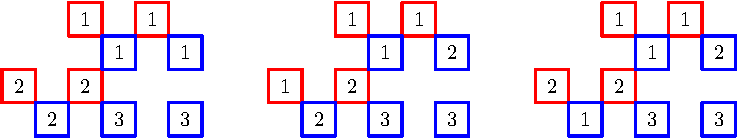
\includegraphics[scale = 0.8]{figures/yamaTableau.pdf}
            \caption{Yamanouchi shuffle tableaux}
            \label{fig:yamaTableau}
        \end{figure}
   \end{exam}

   \begin{rema}
       Shuffle tableaux were originally introduced to study Temperley--Lieb immanants, hence the name Temperley--Lieb crystal. In \cite{nguyen2025temperley}, there are additional constraints on the shapes $\lambda/\mu$ and $\nu/\rho$ so that the crystal operators behave nicely with the Temperley--Lieb type (see Section \ref{subsec:TL-imm}). These constraints are unnecessary for this section.
   \end{rema}

\subsection{Compatible tableaux}

    \begin{defi}[$D$-compatible tableaux]\label{def:compatible}
        Let $D$ be the diagram of $(\lambda/\mu)\circledast(\nu/\rho)$. We label the squares of $D$ $1,2,\ldots,|\lambda/\mu| + |\nu/\rho|$ from right to left, top to bottom. We will refer to the square labeled $i$ as square $i$. A SYT $T$ (of any shape) is $D$-compatible if the following two conditions hold:

        \begin{enumerate}
            \item If square $i+1$ is directly left of square $i$ in $D$, then $i+1$ is weakly North and strictly East of $i$ in $T$. 
            \item If square $i$ is directly above square $j$ in $D$, then $i$ is strictly North and weakly East of $j$ in $T$. 
        \end{enumerate}
    \end{defi}

    \begin{exam}

        Let $D$ be the same diagram as in Example \ref{ex:yama-shuffle-tableau}. The labeling of $D$ from right to left, bottom to top is shown in Figure \ref{fig:compLabelling}. The two SYTs on the left of Figure \ref{fig:compTableau} are $D$-compatible. The SYT on the right is not because 2 is not weakly North of 1, and 2 is not weakly East of 5.

        \begin{figure}[h!]
            \centering
            \begin{minipage}[b]{.4\textwidth}
                \centering
                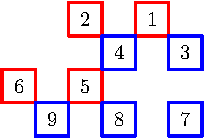
\includegraphics[scale = 0.8]{figures/compLabelling.pdf}
                \caption{Labeling of $D$}
                \label{fig:compLabelling}
            \end{minipage}
            \begin{minipage}[b]{.65\textwidth}
                \centering
                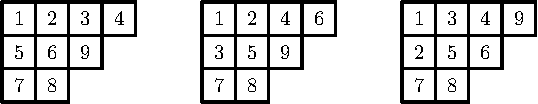
\includegraphics[scale = 0.8]{figures/compTableau.pdf}
                \caption{$D$-compatible tableaux (left and center) and non-$D$-compatible tableau (right)}
                \label{fig:compTableau}
            \end{minipage}
        \end{figure}
    \end{exam}

    Now, we will construct a bijection $\varphi$ between $D$-compatible tableaux and Yamanouchi shuffle tableaux on $D$. Furthermore, for any $D$-compatible tableau $T$, we would like the shape of $T$ to be the same as the content of $\varphi(T)$.

    \begin{defi}[Construction of $\varphi$]\label{def:yama-comp-bijection}
        Given a $D$-compatible tableau $T$, $\varphi(T)$ is constructed as follows: if $i$ is in row $r$ of $T$, then in $\varphi(T)$, put $r$ in square $i$. The inverse of $\varphi$ is also straightforward: given a Yamanouchi shuffle tableau $S$, let $I$ be the set of squares in $S$ that contains $r$, then $I$ is the set of numbers (in increasing order) in row $r$ in $\varphi^{-1}(S)$
    \end{defi}

    For example, the readers may check that $\phi$ sends the two $D$-compatible tableaux to the left of Figure \ref{fig:compTableau} to the two Yamanouchi shuffle tableaux to the left of Figure \ref{fig:yamaTableau}.


    \begin{prop}
        $\varphi$ is a bijection between $D$-compatible tableaux and Yamanouchi shuffle tableaux on $D$ such that for any $D$-compatible tableau $T$, the shape of $T$ is the same as the content of $\varphi(T)$.
    \end{prop}

    \begin{proof}[Proof sketch]
        We will check the following: for any $D$-compatible tableau $T$ and any Yamanouchi shuffle tableau $S$:

        \begin{enumerate}
            \item $\varphi(T)$ is a valid shuffle tableau (Lemma \ref{lem:phiT-valid}),
            \item $\varphi(T)$ is a Yamanouchi shuffle tableau (Lemma \ref{lem:phiT-yama}),
            \item $\varphi^{-1}(S)$ is a valid SYT (Lemma \ref{lem:phiS-valid}),
            \item $\varphi^{-1}(S)$ is $D$-compatible (Lemma \ref{lem:phiS-comp}). \qedhere
        \end{enumerate}
    \end{proof}

    \begin{lemma}\label{lem:phiT-valid}
        For any $D$-compatible tableau $T$, $\varphi(T)$ is a valid shuffle tableau.
    \end{lemma}

    \begin{proof}
        This follows immediately from the compatibility conditions: the rows of $\varphi(T)$ are weakly increasing thanks to condition (1) in Definition \ref{def:compatible}; the columns of $\varphi(T)$ are strictly increasing thanks to condition (2).
    \end{proof}

    \begin{lemma}\label{lem:phiT-yama}
        For any $D$-compatible tableau $T$, $\varphi(T)$ is a Yamanouchi shuffle tableau.
    \end{lemma}

    \begin{proof}
        Suppose for contradiction that square $i$ containing $r$ in $\varphi(T)$ can be lowered by $E_{r-1}$. This means that $r\geq 2$, so in $T$, there is a $j$ directly above $i$. Recall that we say square $(r_1,c_1)$ is right of square $(r_2,c_2)$, and square $(r_2,c_2)$ is left of square $(r_1,c_1)$, if $r_2 > r_1$ or $r_2 = r_1$ and $c_2 < c_1$. Because $T$ is a SYT, in $T$, the number of entries smaller than $j$ on row $r-1$ equals that of entries smaller than $i$ on row $r$.

        In $\varphi(T)$, this means that the number of entries $r-1$ right of square $j$ equals that of entries $r$ right of $i$. Note that $j$ contains an additional $r-1$ right of $i$. On the other hand, $E_{r-1}$ lowers square $i$, so the number of non-$(r-1,r)$-overlapped $r-1$'s right of square $i$ is less than or equal to that of non-$(r-1,r)$-overlapped $r$'s.

        If none of $j$ or the $(r-1)$-squares right of $j$ is $(r-1,r)$-overlapped with $i$ or some $r$-square left of $i$, then we still have the number of non-$(r-1,r)$-overlapped $r-1$'s right of or equal to $j$ is more than that of non-$(r-1,r)$-overlapped $r$ right of $i$. This contradicts the previous paragraph.

        Thus, either $j$ or some $(r-1)$-square right of $j$ has to be $(r-1,r)$-overlapped with either $i$ or some $r$-square left of $i$. Since $E_{r-1}$ lowers square $i$, $i$ cannot be $(r-1,r)$-overlapped. Thus, this $(r-1,r)$-overlap pair has to be $(s,t)$ where $s$ is $j$ or right of $j$, and $t$ is left of $i$.

        This means that in $T$, $t$ is strictly East of $i$, but $s$ is weakly West of $j$ and $i$, which contradicts condition (2) in Definition \ref{def:compatible}.
    \end{proof}

    \begin{lemma}\label{lem:phiS-valid}
        For any Yamanouchi shuffle tableau $S$, $\varphi^{-1}(S)$ is a valid SYT.
    \end{lemma}

    \begin{proof}
        Row strictness follows from the construction. We now check column strictness. Suppose for contradiction that in $\varphi^{-1}(S)$, square $(r,c)$ (row $r$, column $c$) has entry $i$ and square $(r+1,c)$ has entry $j$ where $i > j$. Then, square $j$ in $S$ contains $r+1$. Furthermore, since the rows are sorted in increasing order, there are $c-1$ more squares containing $r+1$ right of $j$. Since $i > j$, there are at most $c-1$ squares containing $r$ right of $j$. Thus, there are at least as many squares containing $r+1$ than $r$ right of $j$ in $S$. Hence, we can apply $E_r$ on $S$, so $S$ is not Yamanouchi, contradiction.
    \end{proof}

    \begin{lemma}\label{lem:phiS-comp}
        For any Yamanouchi shuffle tableau $S$, $\varphi^{-1}(S)$ is $D$-compatible.
    \end{lemma}

    \begin{proof}
        Condition (1) in Definition \ref{def:compatible} follows from $S$ is row increasing and $\varphi^{-1}(S)$ is a valid SYT. We now check condition (2).

        Suppose for contradiction that there are squares $i$ and $j$ in $S$ such that $j$ is directly below $i$, but in $\varphi^{-1}(S)$, $j$ is not strictly South or weakly West of $i$. Note that by column strictness of $S$, $j$ is still strictly South of $i$, so $j$ has to be strictly East of $i$. Let $(s,t)$ be the coordinate of $i$, then $(s+2,t)$ is the coordinate of $j$. Let $r$ be the number in $j$, and $r-k$ be the number in $i$.

        First, we claim that $k \leq 2$. If $k > 2$, in $\varphi^{-1}(S)$, there is $j > h_1>h_2> i$ such that $h_1$ and $h_2$ are directly above $j$, and $h_2$ is strictly Southeast of $i$. Then, in $S$, the squares $j$, $h_1$, $h_2$, and $i$ appears from left to right. However, $j$ contains $r$ on row $s+2$, and $i$ contains $r-k$ on row $s$, but $h_1$ and $h_2$ contains $r-1$ and $r-2$ respectively, so they are both on row $s+1$. This is impossible since $h_1$ is left of $h_2$.

        For the case $k = 2$, we make an extra assumption: among all possible pairs of squares $i,j$ containing $r-2$ and $r$ violating condition (2), choose the pair with $i$ largest possible. Let $h$ be the number directly above $j$ in $\varphi^{-1}(S)$. By the same argument above, in $S$, square $h$ contains $r-1$ and is on row $s+1$. Since $h$ is also strictly East of $i$, there are more $(r-1)$-squares right of $h$ than $(r-2)$-squares right of $i$. Note that none of the $(r-2)$-squares right of $i$ can be $(r-2,r-1)$-overlapped with an $(r-1)$-square left of $h$. This is because such $(r-2)$-square has to be on row $s$, but $i$ is not $(r-2,r-1)$-overlapped, so any $(r-2)$-square left of $i$ on the same row cannot be so either. This means that the number of non-$(r-2,r-1)$-overlapped $(r-2)$-squares right of $i$ is less than that of non-$(r-2,r-1)$-overlapped $(r-1)$-squares right of $h$. Thus, for $S$ to be Yamanouchi, the has to be non-$(r-2,r-1)$-overlapped $(r-2)$-squares right of $h$ but left of $i$. Let $i'$ be such square, then $i' > i$ and $i'$ is also on row $s$. Moreover, the square directly above $i'$, call it $j'$, is on row $s+2$, and $j' > j$. Then, $i'$ and $j'$ is another pair violating condition (2). This contradicts the choice of $i,j$ being such pair with $i$ largest possible.

        Finally, for the case $k = 1$, we also make an (opposite) extra assumption: among all possible pairs of squares $i,j$ containing $r-1$ and $r$ violating condition (2), choose the pair with $i$ smallest possible. Let $h$ be the number directly below $i$ in $\varphi^{-1}(S)$, then $h$ contains $r$ and is on row $s+1$. By the choice of $i$, $h$ is not $(r-1,r)$-overlapped, and neither is any $r$-square right of $j$ on row $s+2$. Since $h$ is directly above $i$ in $\varphi^{-1}(S)$, in $S$, there are as many $(r-1)$-squares right of $i$ as $r$-squares right of $h$. Any $(r-1)$-square right of $i$ on row $s$ cannot be $(r-1,r)$-overlapped by the choice of $i$. Hence, there are as many non-$(r-1,r)$-overlapped $(r-1)$-squares right of $i$ as non-$(r-1,r)$-overlapped $r$-squares right of $h$. On the other hand, any $(r-1)$-square left of $i$ but right of $h$, including $i$, is on row $s$ and is $(r-1,r)$-overlapped. Thus, to the right of $h$, there are as many non-$(r-1,r)$-overlapped $(r-1)$-squares as $r$-squares. However, $h$ is itself non-$(r-1,r)$-overlapped, so $S$ is not Yamanouchi. This contradiction completes the proof.
    \end{proof}

% Reference facts from the official published article HTML; citation keys and printed numbers recovered from the published PDF named destinations.
\begin{thebibliography}{99}
\bibitem[1]{BB} Beĭlinson, Alexandre; Bernstein, Joseph Localisation de $g$-modules, C. R. Acad. Sci. Paris Sér. I Math., Volume 292 (1981) no. 1, pp. 15-18.
\bibitem[2]{benderknuth1972} Bender, Edward A.; Knuth, Donald E. Enumeration of plane partitions, J. Combinatorial Theory Ser. A, Volume 13 (1972), pp. 40-54 \url{https://doi.org/10.1016/0097-3165(72)90007-6}.
\bibitem[3]{berenstein-zelevenski} Berenshteĭn, A. D.; Zelevinskiĭ, A. V. When is the multiplicity of a weight equal to $1$?, Funktsional. Anal. i Prilozhen., Volume 24 (1990) no. 4, p. 1-13, 96 \url{https://doi.org/10.1007/BF01077330}.
\bibitem[4]{berenstein-kirilov} Berenstein, A. D.; Kirillov, A. N. Groups generated by involutions, Gelfand-Tsetlin patterns, and combinatorics of Young tableaux, Algebra i Analiz, Volume 7 (1995) no. 1, pp. 92-152.
\bibitem[5]{berenstein1992triple} Berenstein, A. D.; Zelevinsky, A. V. Triple multiplicities for ${\rm sl}(r+1)$ and the spectrum of the exterior algebra of the adjoint representation, J. Algebraic Combin., Volume 1 (1992) no. 1, pp. 7-22 \url{https://doi.org/10.1023/A:1022429213282}.
\bibitem[6]{berenstein1996parametrizations} Berenstein, Arkady; Fomin, Sergey; Zelevinsky, Andrei Parametrizations of canonical bases and totally positive matrices, Adv. Math., Volume 122 (1996) no. 1, pp. 49-149 \url{https://doi.org/10.1006/aima.1996.0057}.
\bibitem[7]{berenstein1999tensor} Berenstein, Arkady; Zelevinsky, Andrei Tensor product multiplicities, canonical bases and totally positive varieties, Invent. Math., Volume 143 (2001) no. 1, pp. 77-128 \url{https://doi.org/10.1007/s002220000102}.
\bibitem[8]{bergeron2004some} Bergeron, François; McNamara, Peter Some positive differences of products of Schur functions, 2004.
\bibitem[9]{brylinski1981kazhdan} Brylinski, J.-L.; Kashiwara, M. Kazhdan-Lusztig conjecture and holonomic systems, Invent. Math., Volume 64 (1981) no. 3, pp. 387-410 \url{https://doi.org/10.1007/BF01389272}.
\bibitem[10]{chiang2024bender} Chiang, Judy Hsin-Hui; Hoang, Anh Trong Nam; Kendall, Matthew; Lynch, Ryan; Nguyen, Son; Przybocki, Benjamin; Xia, Janabel Bender-Knuth involutions on linear extensions of posets, Discrete Math., Volume 347 (2024) no. 9, Paper no. 114068, 20 pages \url{https://doi.org/10.1016/j.disc.2024.114068}.
\bibitem[11]{CGP} Chmutov, Michael; Glick, Max; Pylyavskyy, Pavlo The Berenstein-Kirillov group and cactus groups, J. Comb. Algebra, Volume 4 (2020) no. 2, pp. 111-140 \url{https://doi.org/10.4171/JCA/36}.
\bibitem[12]{dobrovolska2007products} Dobrovolska, Galyna; Pylyavskyy, Pavlo On products of $\mathfrak{sl}_{\mathfrak{n}}$ characters and support containment, J. Algebra, Volume 316 (2007) no. 2, pp. 706-714 \url{https://doi.org/10.1016/j.jalgebra.2006.10.033}.
\bibitem[13]{du1992canonical} Du, Jie Canonical bases for irreducible representations of quantum ${\rm {GL}}_n$, Bull. London Math. Soc., Volume 24 (1992) no. 4, pp. 325-334 \url{https://doi.org/10.1112/blms/24.4.325}.
\bibitem[14]{du1995canonical} Du, Jie Canonical bases for irreducible representations of quantum ${\rm {GL}}_n$. II, J. London Math. Soc. (2), Volume 51 (1995) no. 3, pp. 461-470 \url{https://doi.org/10.1112/jlms/51.3.461}.
\bibitem[15]{fomin2005eigenvalues} Fomin, Sergey; Fulton, William; Li, Chi-Kwong; Poon, Yiu-Tung Eigenvalues, singular values, and Littlewood-Richardson coefficients, Amer. J. Math., Volume 127 (2005) no. 1, pp. 101-127 \url{https://doi.org/10.1353/ajm.2005.0005}.
\bibitem[16]{fomin2002cluster} Fomin, Sergey; Zelevinsky, Andrei Cluster algebras. I. Foundations, J. Amer. Math. Soc., Volume 15 (2002) no. 2, pp. 497-529 \url{https://doi.org/10.1090/S0894-0347-01-00385-X}.
\bibitem[17]{haiman1993hecke} Haiman, Mark Hecke algebra characters and immanant conjectures, J. Amer. Math. Soc., Volume 6 (1993) no. 3, pp. 569-595 \url{https://doi.org/10.2307/2152777}.
\bibitem[18]{kashiwara1991crystal} Kashiwara, Masaki On crystal bases of the ${Q}$-analogue of universal enveloping algebras, Duke Math. J., Volume 63 (1991) no. 2, pp. 465-516 \url{https://doi.org/10.1215/S0012-7094-91-06321-0}.
\bibitem[19]{kashiwara1993global} Kashiwara, Masaki Global crystal bases of quantum groups, Duke Math. J., Volume 69 (1993) no. 2, pp. 455-485 \url{https://doi.org/10.1215/S0012-7094-93-06920-7}.
\bibitem[20]{knutson1999honeycomb} Knutson, Allen; Tao, Terence The honeycomb model of ${\rm {GL}}_n({\bf {C}})$ tensor products. I. Proof of the saturation conjecture, J. Amer. Math. Soc., Volume 12 (1999) no. 4, pp. 1055-1090 \url{https://doi.org/10.1090/S0894-0347-99-00299-4}.
\bibitem[21]{lam2007alcoved} Lam, Thomas; Postnikov, Alexander Alcoved polytopes. I, Discrete Comput. Geom., Volume 38 (2007) no. 3, pp. 453-478 \url{https://doi.org/10.1007/s00454-006-1294-3}.
\bibitem[22]{lam2018alcoved} Lam, Thomas; Postnikov, Alexander Alcoved polytopes II, Lie groups, geometry, and representation theory (Progr. Math.), Volume 326, Birkhäuser/Springer, Cham, 2018, pp. 253-272 \url{https://doi.org/10.1007/978-3-030-02191-7_10}.
\bibitem[23]{lam2007schur} Lam, Thomas; Postnikov, Alexander; Pylyavskyy, Pavlo Schur positivity and Schur log-concavity, Amer. J. Math., Volume 129 (2007) no. 6, pp. 1611-1622 \url{https://doi.org/10.1353/ajm.2007.0045}.
\bibitem[24]{lascoux1997ribbon} Lascoux, Alain; Leclerc, Bernard; Thibon, Jean-Yves Ribbon tableaux, Hall-Littlewood functions, quantum affine algebras, and unipotent varieties, J. Math. Phys., Volume 38 (1997) no. 2, pp. 1041-1068 \url{https://doi.org/10.1063/1.531807}.
\bibitem[25]{littlewood1934group} Littlewood, Dudley Ernest; Richardson, Archibald Read Group characters and algebra, Philosophical Transactions of the Royal Society of London. Series A, Containing Papers of a Mathematical or Physical Character, Volume 233 (1934) no. 721-730, pp. 99-141 \url{https://doi.org/10.1098/rsta.1934.0015}.
\bibitem[26]{lusztig1990canonical} Lusztig, George Canonical bases arising from quantized enveloping algebras, J. Amer. Math. Soc., Volume 3 (1990) no. 2, pp. 447-498 \url{https://doi.org/10.2307/1990961}.
\bibitem[27]{lusztig1994total} Lusztig, George Total positivity in reductive groups, Lie theory and geometry (Progr. Math.), Volume 123, Birkhäuser Boston, Boston, MA, 1994, pp. 531-568 \url{https://doi.org/10.1007/978-1-4612-0261-5_20}.
\bibitem[28]{lusztig1997total} Lusztig, George Total positivity and canonical bases, Algebraic groups and Lie groups (Austral. Math. Soc. Lect. Ser.), Volume 9, Cambridge Univ. Press, Cambridge, 1997, pp. 281-295.
\bibitem[29]{nguyen2023cactus} Nguyen, Son The Cactus Group Property for Ordinal Sums of Disjoint Unions of Chains, 2023.
\bibitem[30]{nguyen2025temperley} Nguyen, Son; Pylyavskyy, Pavlo Temperley-Lieb crystals, Int. Math. Res. Not. IMRN (2025) no. 7, Paper no. rnaf080, 28 pages \url{https://doi.org/10.1093/imrn/rnaf080}.
\bibitem[31]{okounkov1997log} Okounkov, Andrei Log-concavity of multiplicities with application to characters of ${\rm {U}}(\infty )$, Adv. Math., Volume 127 (1997) no. 2, pp. 258-282 \url{https://doi.org/10.1006/aima.1997.1622}.
\bibitem[32]{pylyavskyy2007comparing} Pylyavskyy, Pavlo Comparing products of Schur functions and quasisymmetric functions, Ph. D. Thesis, Massachusetts Institute of Technology (2007).
\bibitem[33]{reiner1998percentage} Reiner, Victor; Shimozono, Mark Percentage-avoiding, northwest shapes and peelable tableaux, J. Combin. Theory Ser. A, Volume 82 (1998) no. 1, pp. 1-73 \url{https://doi.org/10.1006/jcta.1997.2841}.
\bibitem[34]{remmel1984multiplying} Remmel, J. B.; Whitney, R. Multiplying Schur functions, J. Algorithms, Volume 5 (1984) no. 4, pp. 471-487 \url{https://doi.org/10.1016/0196-6774(84)90002-6}.
\bibitem[35]{rhoades2005temperley} Rhoades, Brendon; Skandera, Mark Temperley-Lieb immanants, Ann. Comb., Volume 9 (2005) no. 4, pp. 451-494 \url{https://doi.org/10.1007/s00026-005-0268-0}.
\bibitem[36]{rhoades2006kazhdan} Rhoades, Brendon; Skandera, Mark Kazhdan-Lusztig immanants and products of matrix minors, J. Algebra, Volume 304 (2006) no. 2, pp. 793-811 \url{https://doi.org/10.1016/j.jalgebra.2005.07.017}.
\bibitem[37]{SCHUTZENBERGER1972} Schützenberger, M. P. Promotion des morphismes d’ensembles ordonnés, Discrete Math., Volume 2 (1972), pp. 73-94 \url{https://doi.org/10.1016/0012-365X(72)90062-3}.
\bibitem[38]{skandera2008dual} Skandera, Mark On the dual canonical and Kazhdan-Lusztig bases and 3412-, 4231-avoiding permutations, J. Pure Appl. Algebra, Volume 212 (2008) no. 5, pp. 1086-1104 \url{https://doi.org/10.1016/j.jpaa.2007.09.007}.
\bibitem[39]{zelevinsky1981generalization} Zelevinsky, A. V. A generalization of the Littlewood-Richardson rule and the Robinson-Schensted-Knuth correspondence, J. Algebra, Volume 69 (1981) no. 1, pp. 82-94 \url{https://doi.org/10.1016/0021-8693(81)90128-9}.
\end{thebibliography}
\end{document}
